\Subsubsubsection{Potencia}
Para la unidad de potencia se utilizaran paneles solares y una batería de gel de ciclo profundo conectados a la  placa DFR0580  la cual se encarga de cargar la batería con los paneles solares y asegurar 4 salidas de tension:
\begin{itemize}
\item 5V 2.5A [USB] x 2
\item 5V 5A x 1 
\item 12V 8A x 1
\end{itemize} ,
Con estas salidas se alimentara todos los módulos,excepto por el oscilador de potencia, para este se necesita una etapa DC-DC para elevar la tensi\'on.
Esta etapa es una fuente switching de topolog\'ia Boost.



\Subsubsubsection{Cargador}
Para la etapa del cargador, la transmisión inalámbrica va a constar: del lado del transmisor, de un oscilador en 915Mhz que est\'a comandado por la RPi, y un amplificador de potencia alimentado por un DC/DC de 12V a 15V.

Por el lado del receptor, se encuentra el integrado P1110B que estabiliza la energía para proveer realizar la carga de al UBM.

\begin{figure}[H]
	\centering
	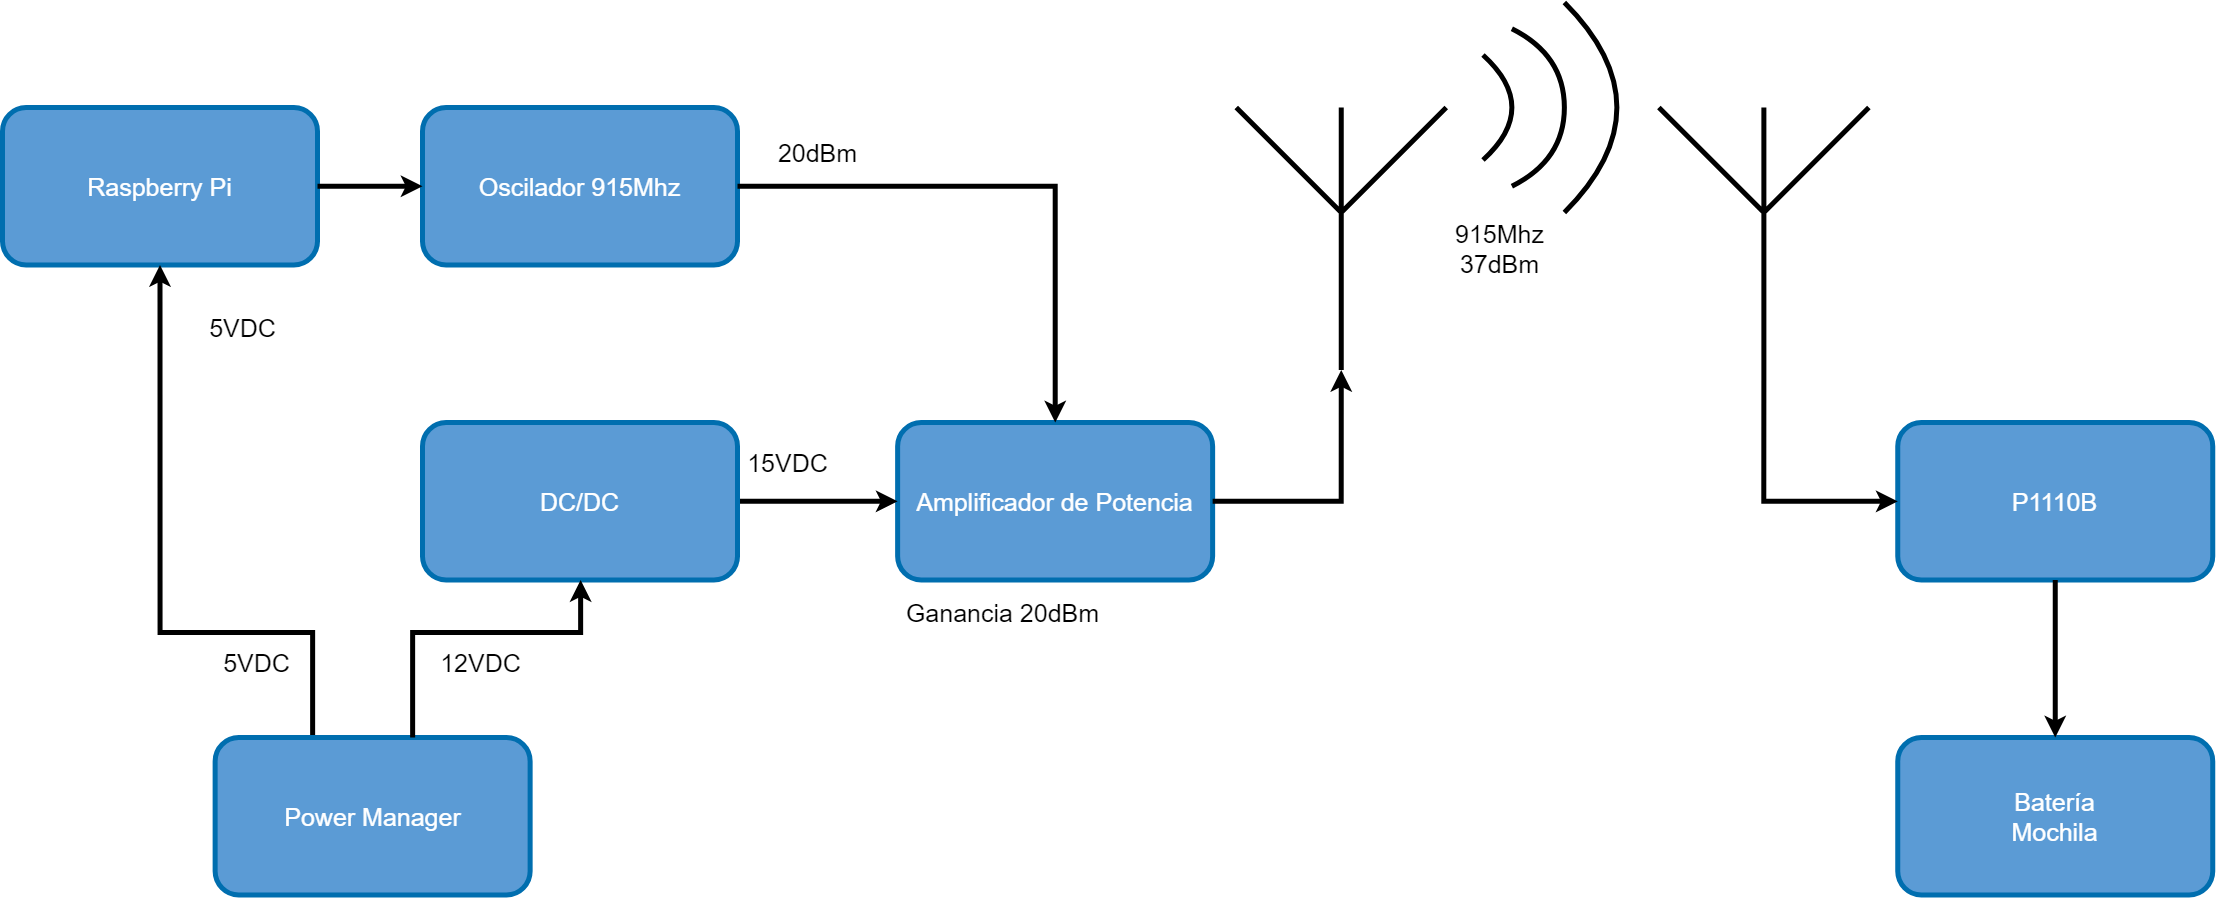
\includegraphics[width=0.9\linewidth]{ImagenesIngenieria de Detalle/EsquemaHardwareAntenas}
	\label{fig:diagrama_hardware_antenas}
	\caption{Diagrama en bloques cargador.}
\end{figure}

\Subsubsubsection{Sensado}
En esta secci\'on aparte del conexionado de los sensores haremos detalle en los pines de la raspberry pi que ser\'an utilizados.
\begin{figure}[H]
	\centering
	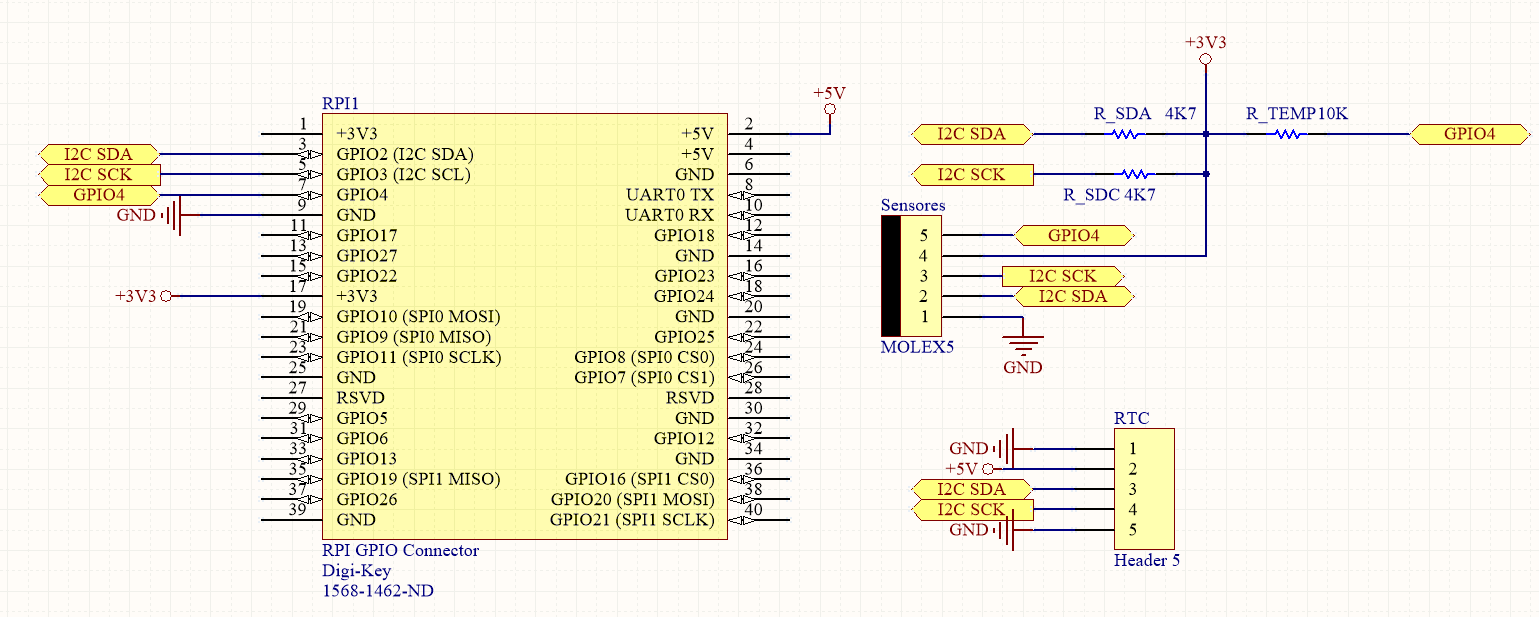
\includegraphics[width=0.9\linewidth]{ImagenesIngenieria de Detalle/Conexionado_rpi}
	\label{fig:conexionado_Rpi}
	\caption{Conexionado Raspberry Pi.}
\end{figure}
El sensor de humedad y temperatura DHT-22 se comunica de manera serial a través de un pin de GPIO.
Para que esto sea posible el sensor necesita 3.3V, GND y el pin de GPIO por donde se realiza la  comunicación, teniendo en cuenta que es necesario un pull-up entre la linea de datos y 3.3V.

El oscilador necesita alimentación, tierra y su comunicación utilizá el protocolo UART.

La cámara simplemente se conecta al zócalo destinado para este próposito en la placa.

Además se tiene un pin de GPIO el cual indicará el momento de prendido del cargador.

Para el conexionado con el sensor de luminosidad y RTC se utilizará el protocolo de comunicación $I^2C$ en modo multi-slave

\begin{figure}[H]
	\centering
	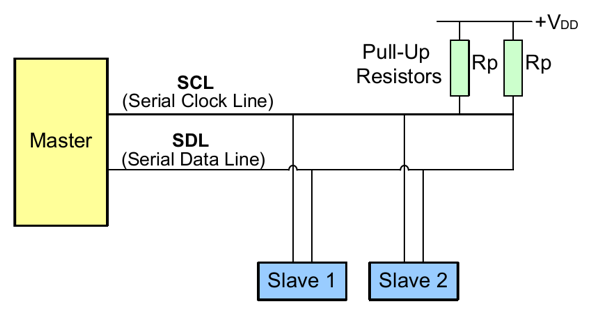
\includegraphics[width=0.7\linewidth]{ImagenesIngenieria de Detalle/I2C_conexionado}
	\label{fig:conexionado_i2c}
	\caption{Conexionado $I^2C$ Multi-slave.}
\end{figure}


